\documentclass{standalone}

\usepackage{tikz}

\usetikzlibrary{shapes.geometric}
\begin{document}
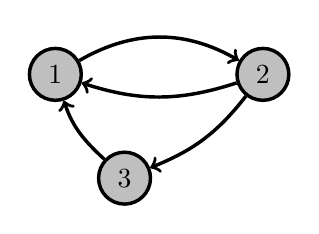
\begin{tikzpicture}
[every node/.style={inner sep=0pt}]
\node (1) [circle, minimum size=18.75pt, fill=lightgray, line width=1.25pt, draw=black] at (25.0pt, -37.5pt) {\textcolor{black}{1}};
\node (2) [circle, minimum size=18.75pt, fill=lightgray, line width=1.25pt, draw=black] at (100.0pt, -37.5pt) {\textcolor{black}{2}};
\node (3) [circle, minimum size=18.75pt, fill=lightgray, line width=1.25pt, draw=black] at (50.0pt, -75.0pt) {\textcolor{black}{3}};
\draw [line width=1.25, ->, color=black] (1) to  [in=150, out=30] (2);
\draw [line width=1.25, ->, color=black] (2) to  [in=342, out=198] (1);
\draw [line width=1.25, ->, color=black] (3) to  [in=288, out=137] (1);
\draw [line width=1.25, ->, color=black] (2) to  [in=22, out=232] (3);
\end{tikzpicture}
\end{document}
